%!TEX root=main.tex
\subsection{Skip Connection}
\label{sec:skip_conn}

Skip connection, as one of the most important techniques to enable training deep networks, also has significant effect to the loss landscape. 
As mentioned in \cite{li2018visualizing}, the skip connections are able to bring smoother loss surface after training. 

\begin{figure}[htp]
	\begin{tabular}{cc}
		\subfloat[With Skip Connection]{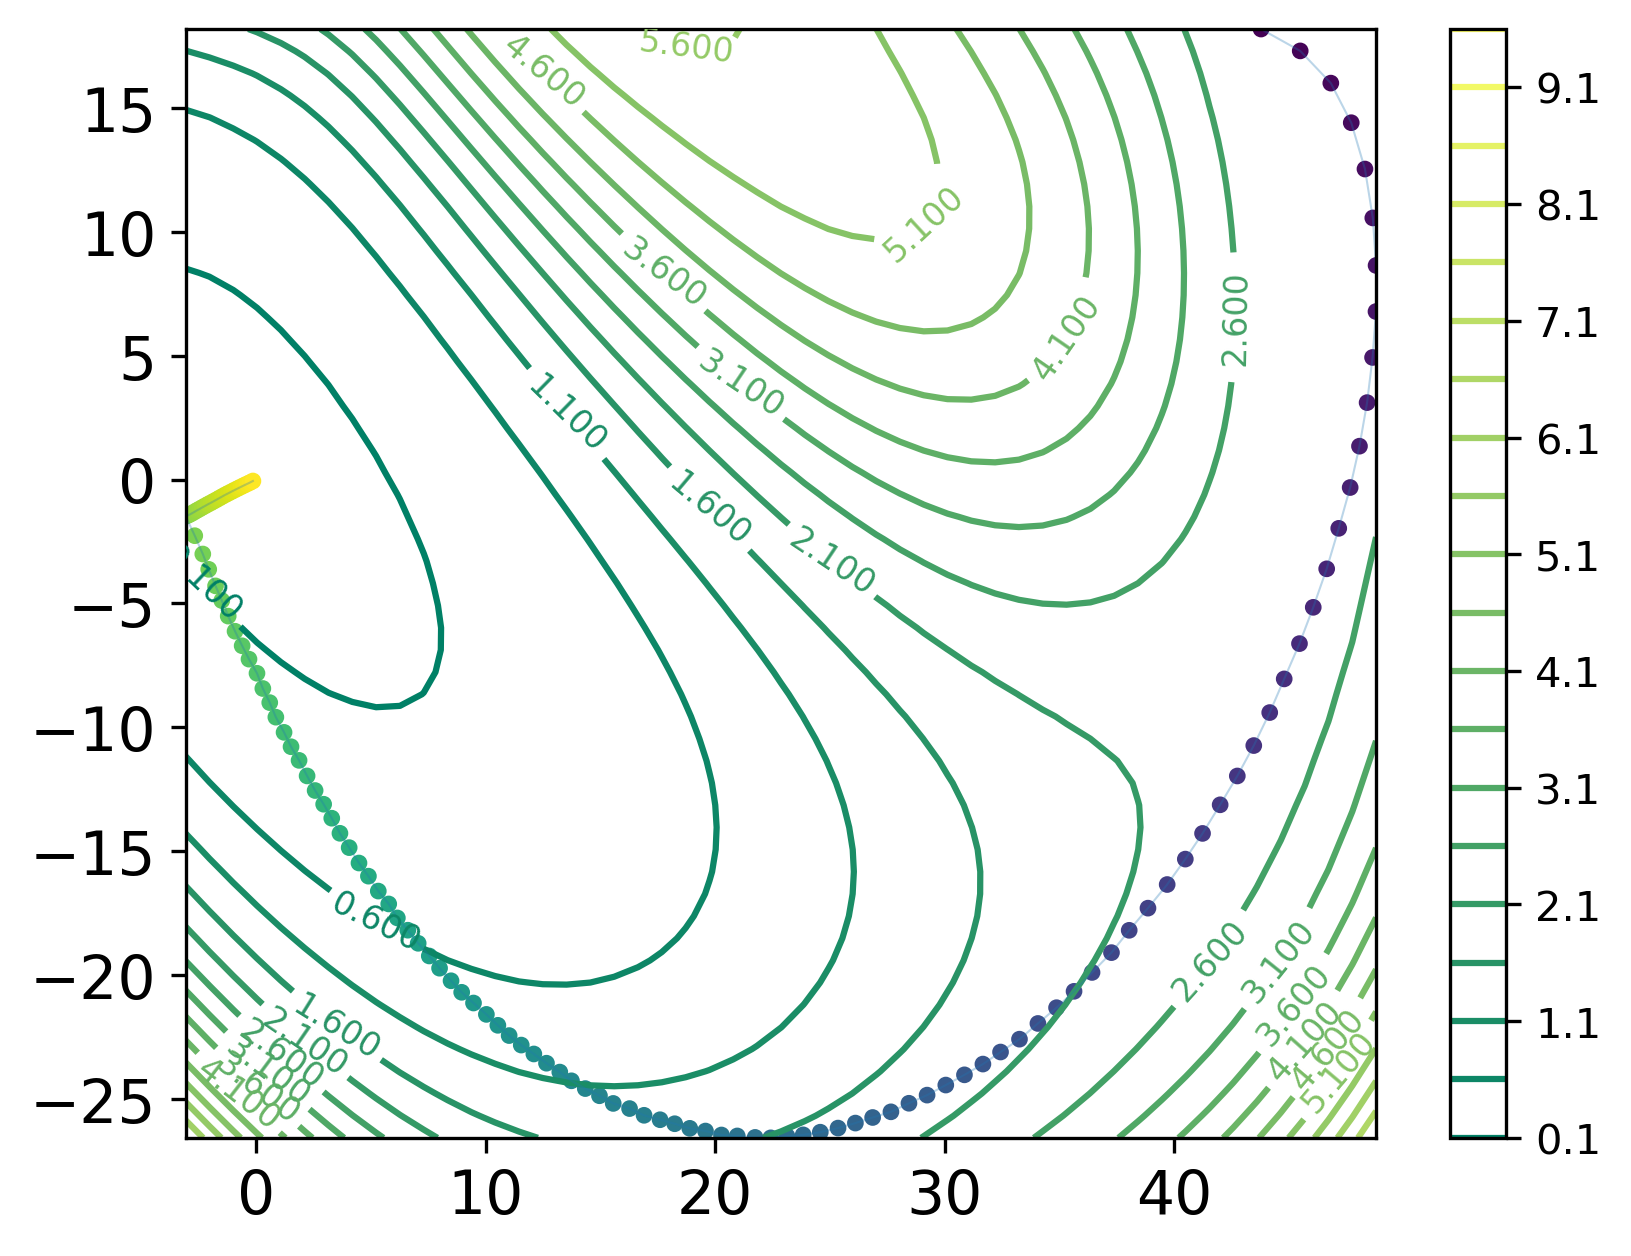
\includegraphics[width =  0.45\linewidth]{results/skip_conn/with_trajectory+contour.png}} &
		\subfloat[Without Skip Connection]{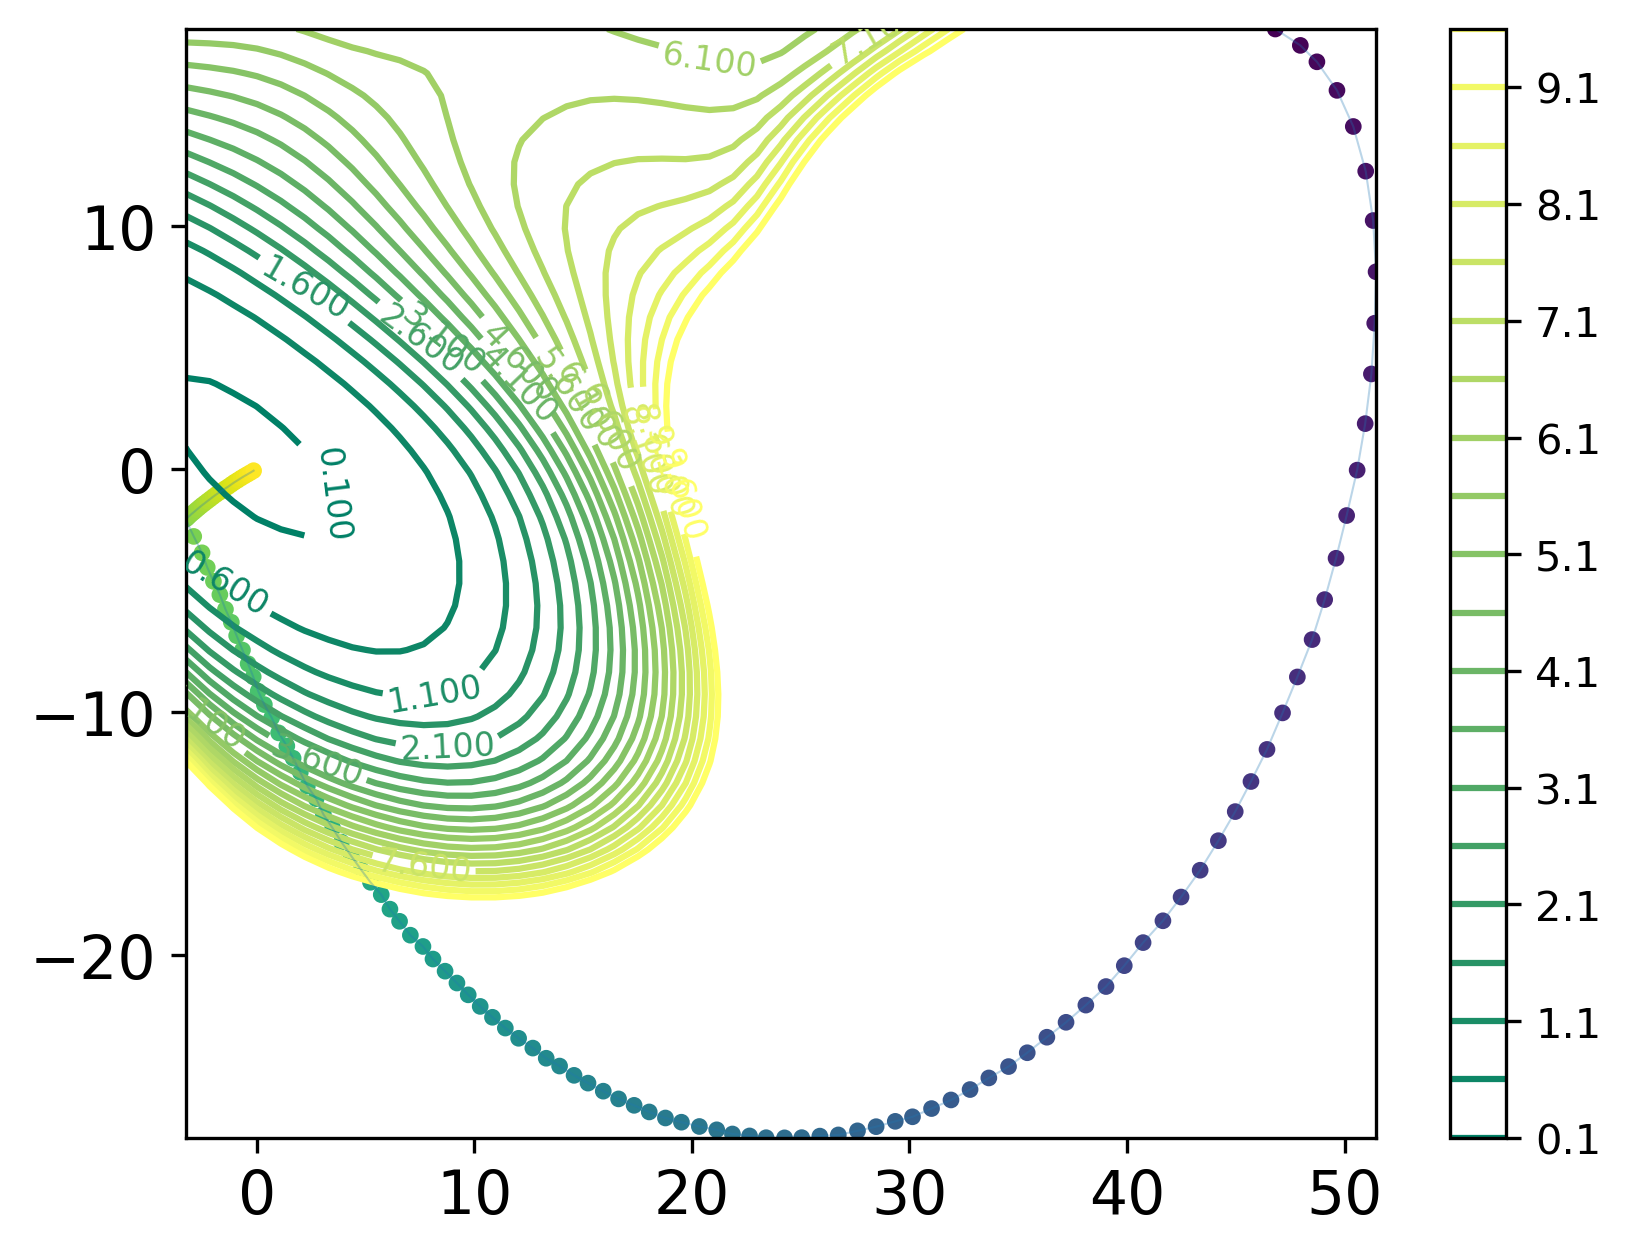
\includegraphics[width =  0.45\linewidth]{results/skip_conn/without_trajectory+contour.png}} 
	\end{tabular}
	\caption{Loss landscapes with/without Skip Connection (Trained)}
	\label{fig:skip-conn-final}
\end{figure}

%However, how does the landscape look at the initialization for these architectures?
Clearly, our results in \pref{fig:skip-conn-final} support their claims of the trained networks.  
Then, a natural question arise: would the skip connections ensure the smoother loss surface even prior to training?
In other words, instead of being benign to the training process, do the skip connections improve the smoothness of loss surface? 

Our results presented in \pref{fig:skip-conn-init} answer the question affirmatively. 
We visual the loss landscapes for the initialized weights with the same directions for projection as in \pref{fig:skip-conn-final}. 
As one can verify that, the loss surface with skip connections is smoother than the other one, as the contour lines are less dense. 
On the other hand, compared with \pref{fig:skip-conn-final}, the difference between loss landscapes with/without skip connections is less prominent. 
This probably indicates that, during the training time, the skip connections improve the propagation of information throughout the neural networks from shallow layers to deep layers, thus help the weights to be updated in a stable manner where the loss surface is turned to be more ``flat''.

\begin{figure}[htp]
	\begin{tabular}{cc}
		\subfloat[With Skip Connection]{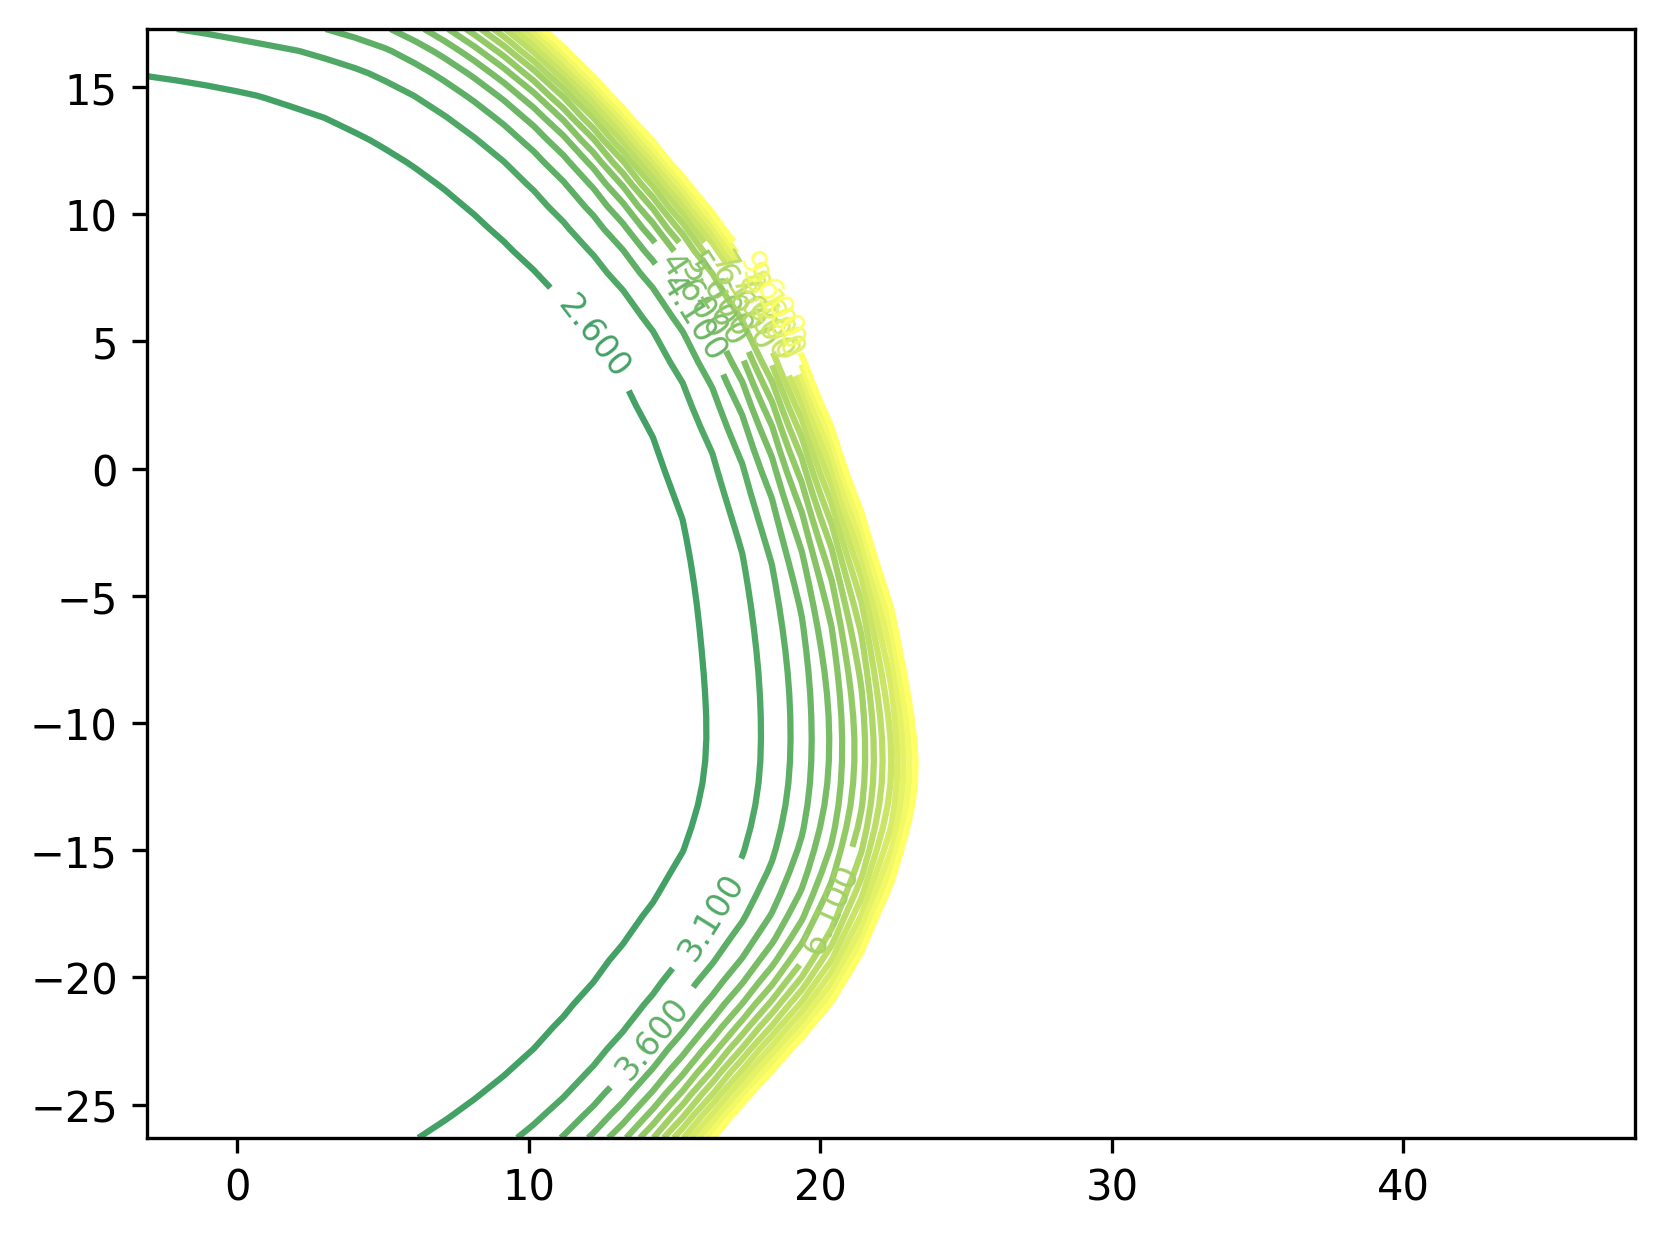
\includegraphics[width =  0.45\linewidth]{results/skip_conn_init/with_contour.png}} &
		\subfloat[Without Skip Connection]{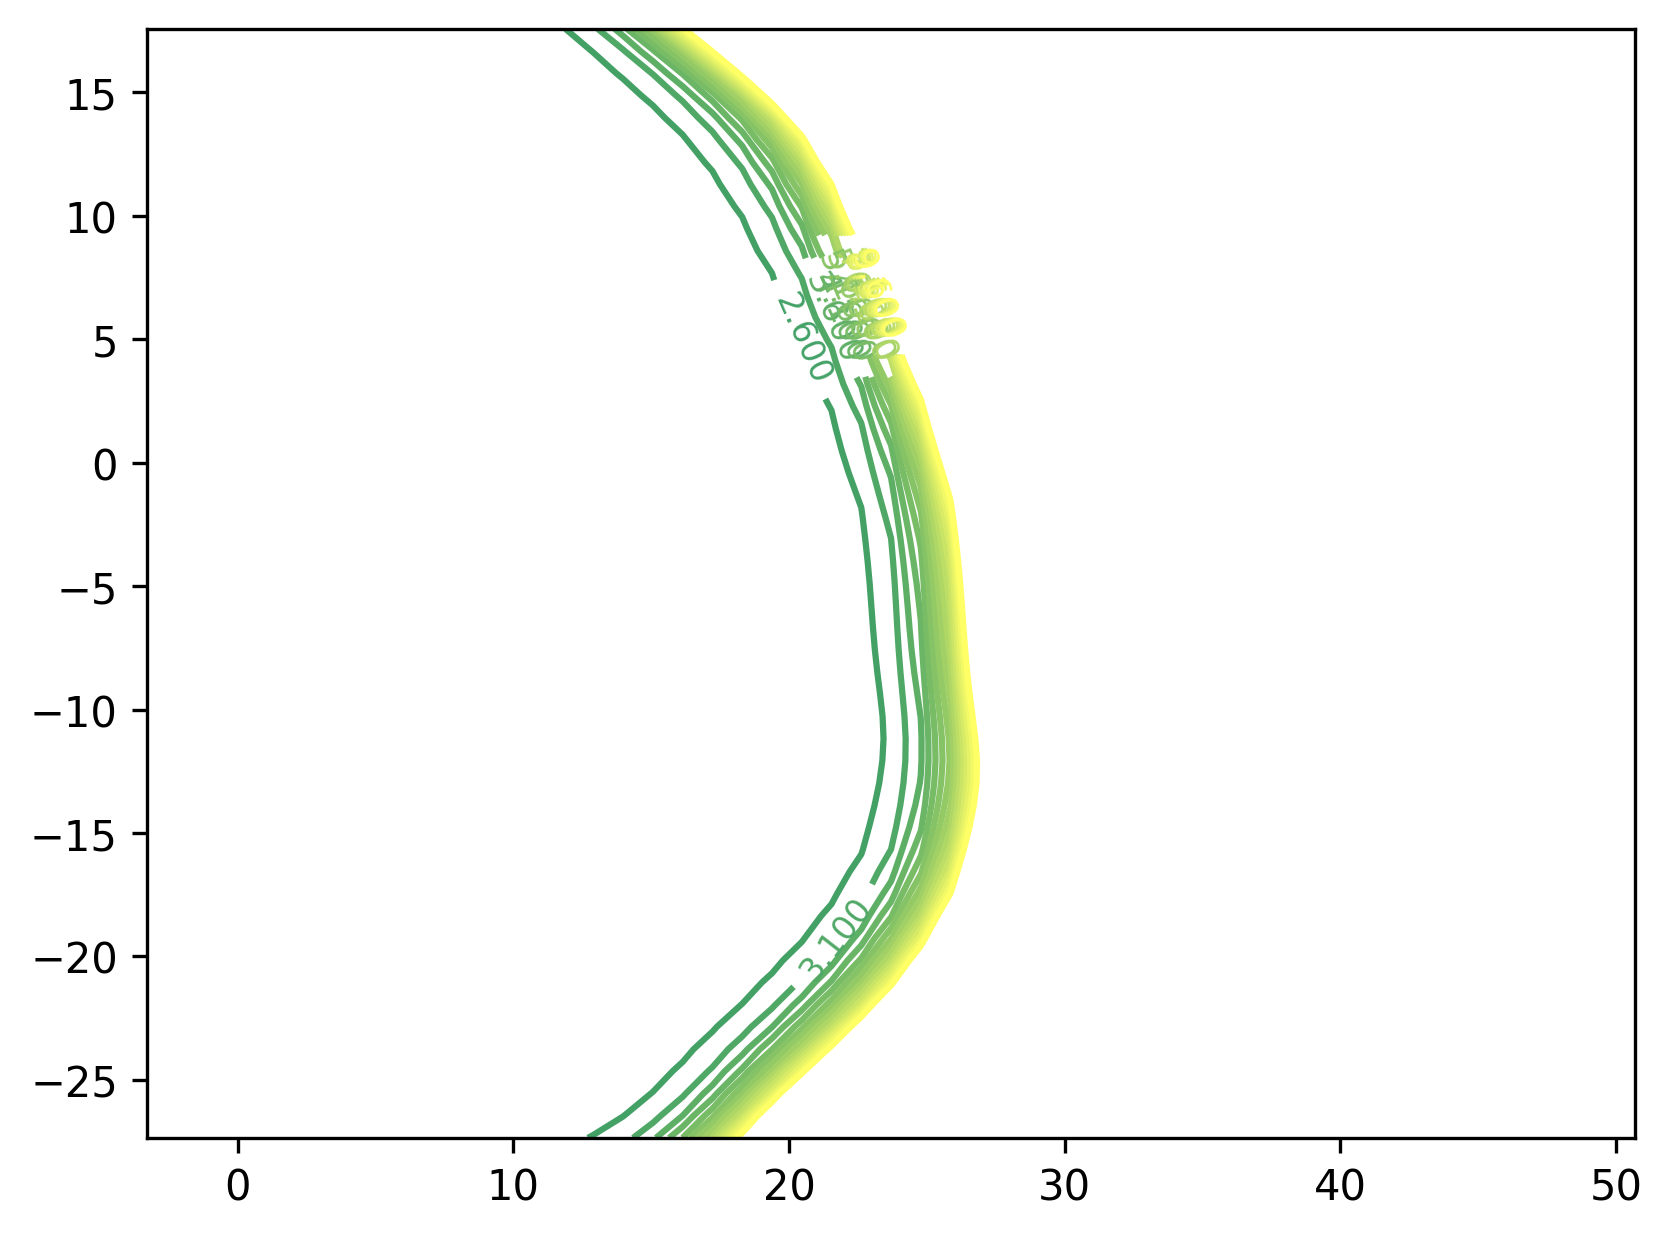
\includegraphics[width =  0.45\linewidth]{results/skip_conn_init/without_contour.png}} 
	\end{tabular}
	\caption{Loss landscapes with/without Skip Connection (Initialized)}
	\label{fig:skip-conn-init}
\end{figure}


